\chapter{Svolgimento dello \textit{stage}}
    \section{Conoscenza del dominio di applicazione}
    La fase iniziale del progetto ha previsto un'immersione approfondita nel dominio applicativo, costituito da un ecosistema manifatturiero dedicato alla produzione di beni per aziende terze. Il sistema in esame si configura come una soluzione trasversale e implementabile in molteplici realtà produttive che adottano metodologie operative simili. L'architettura attuale è basata sulla piattaforma SAI, mentre l'obiettivo dello \textit{stage} è stato quello di condurre un'analisi completa finalizzata alla rimodellazione del dominio.

    \vspace{0.2 em}
    \noindent Le caratteristiche principali del sistema attuale sono:

    \begin{itemize}
        \item \textbf{tracciabilità delle risorse umane}: il sistema mantiene un registro completo del personale operativo, con identificazione univoca di ciascun lavoratore all'interno dell'ecosistema informativo;

        \item \textbf{monitoraggio del processo produttivo}: ogni fase della catena di lavorazione è dettagliatamente documentata, con registrazione sistematica dello stato avanzamento lavori per ciascuna operazione in corso;

        \item \textbf{gestione dell'inventario}: implementazione di meccanismi di controllo delle materie prime, con funzionalità di rilevamento delle soglie critiche e conseguente attivazione di processi di approvvigionamento, alcuni dei quali completamente automatizzati;

        \item \textbf{amministrazione integrata}: il sistema incorpora moduli per la gestione contabile, l'elaborazione documentale e la pianificazione logistica del trasporto.

    \end{itemize}
    
    \vspace{0.2 em}
    \noindent Il progetto di \textit{stage} si è focalizzato principalmente sull’analisi approfondita del dominio applicativo, con l’obiettivo di aggiornare e ridefinire il modello esistente. Questo processo ha previsto l’identificazione e la delimitazione dei \textit{bounded contexts} secondo i principi del \textit{Domain-Driven Design}, cercando di mantenere una rappresentazione chiara e coerente delle diverse aree funzionali del sistema. La fase successiva ha riguardato la formalizzazione dei requisiti funzionali e non funzionali, definendo così i confini tecnici e prestazionali necessari per sviluppare un’eventuale reingegnerizzazione del sistema attualmente basato sulla piattaforma SAI. Come anticipato nella Sezione 1.6.2, le situazioni descritte possono costituire un modello di dominio completo.  

    \vspace{0.2 em}
    \noindent L’obiettivo principale del progetto di \textit{stage} era individuare un modello di dominio specifico e svilupparne un prototipo. Dopo un’attenta valutazione, è stato scelto il \textbf{monitoraggio del processo produttivo} come ambito di intervento. Durante il lavoro, ho potuto constatare quanto sia complesso separare completamente i modelli di dominio, poiché alcuni si intersecano inevitabilmente. Questo mi ha portato alla consapevolezza che non esiste una soluzione perfetta in senso assoluto, ma piuttosto un compromesso tra le diverse esigenze e realtà operative. 
    
    
    \section{Attività svolte}
        \subsection{Analisi dei requisiti}
        Tra i vari modelli di dominio individuati, è stato dunque selezionato quello relativo al \textbf{monitoraggio del processo produttivo}, il quale rientra nell’ambito dell’analisi dei requisiti, come descritto nella Sezione 1.6.1. 

        \vspace{0.2 em}
        \noindent L’analisi dei requisiti è stata condotta in collaborazione con il \textit{Product Owner}, partendo dall’esame approfondito della situazione rappresentata nell’Immagine \ref{fig:Dominio}. Tale attività ha permesso di delineare con precisione le necessità operative e gli obiettivi funzionali, costituendo la base per lo sviluppo del prototipo.

        \begin{figure}[H]
            \centering
            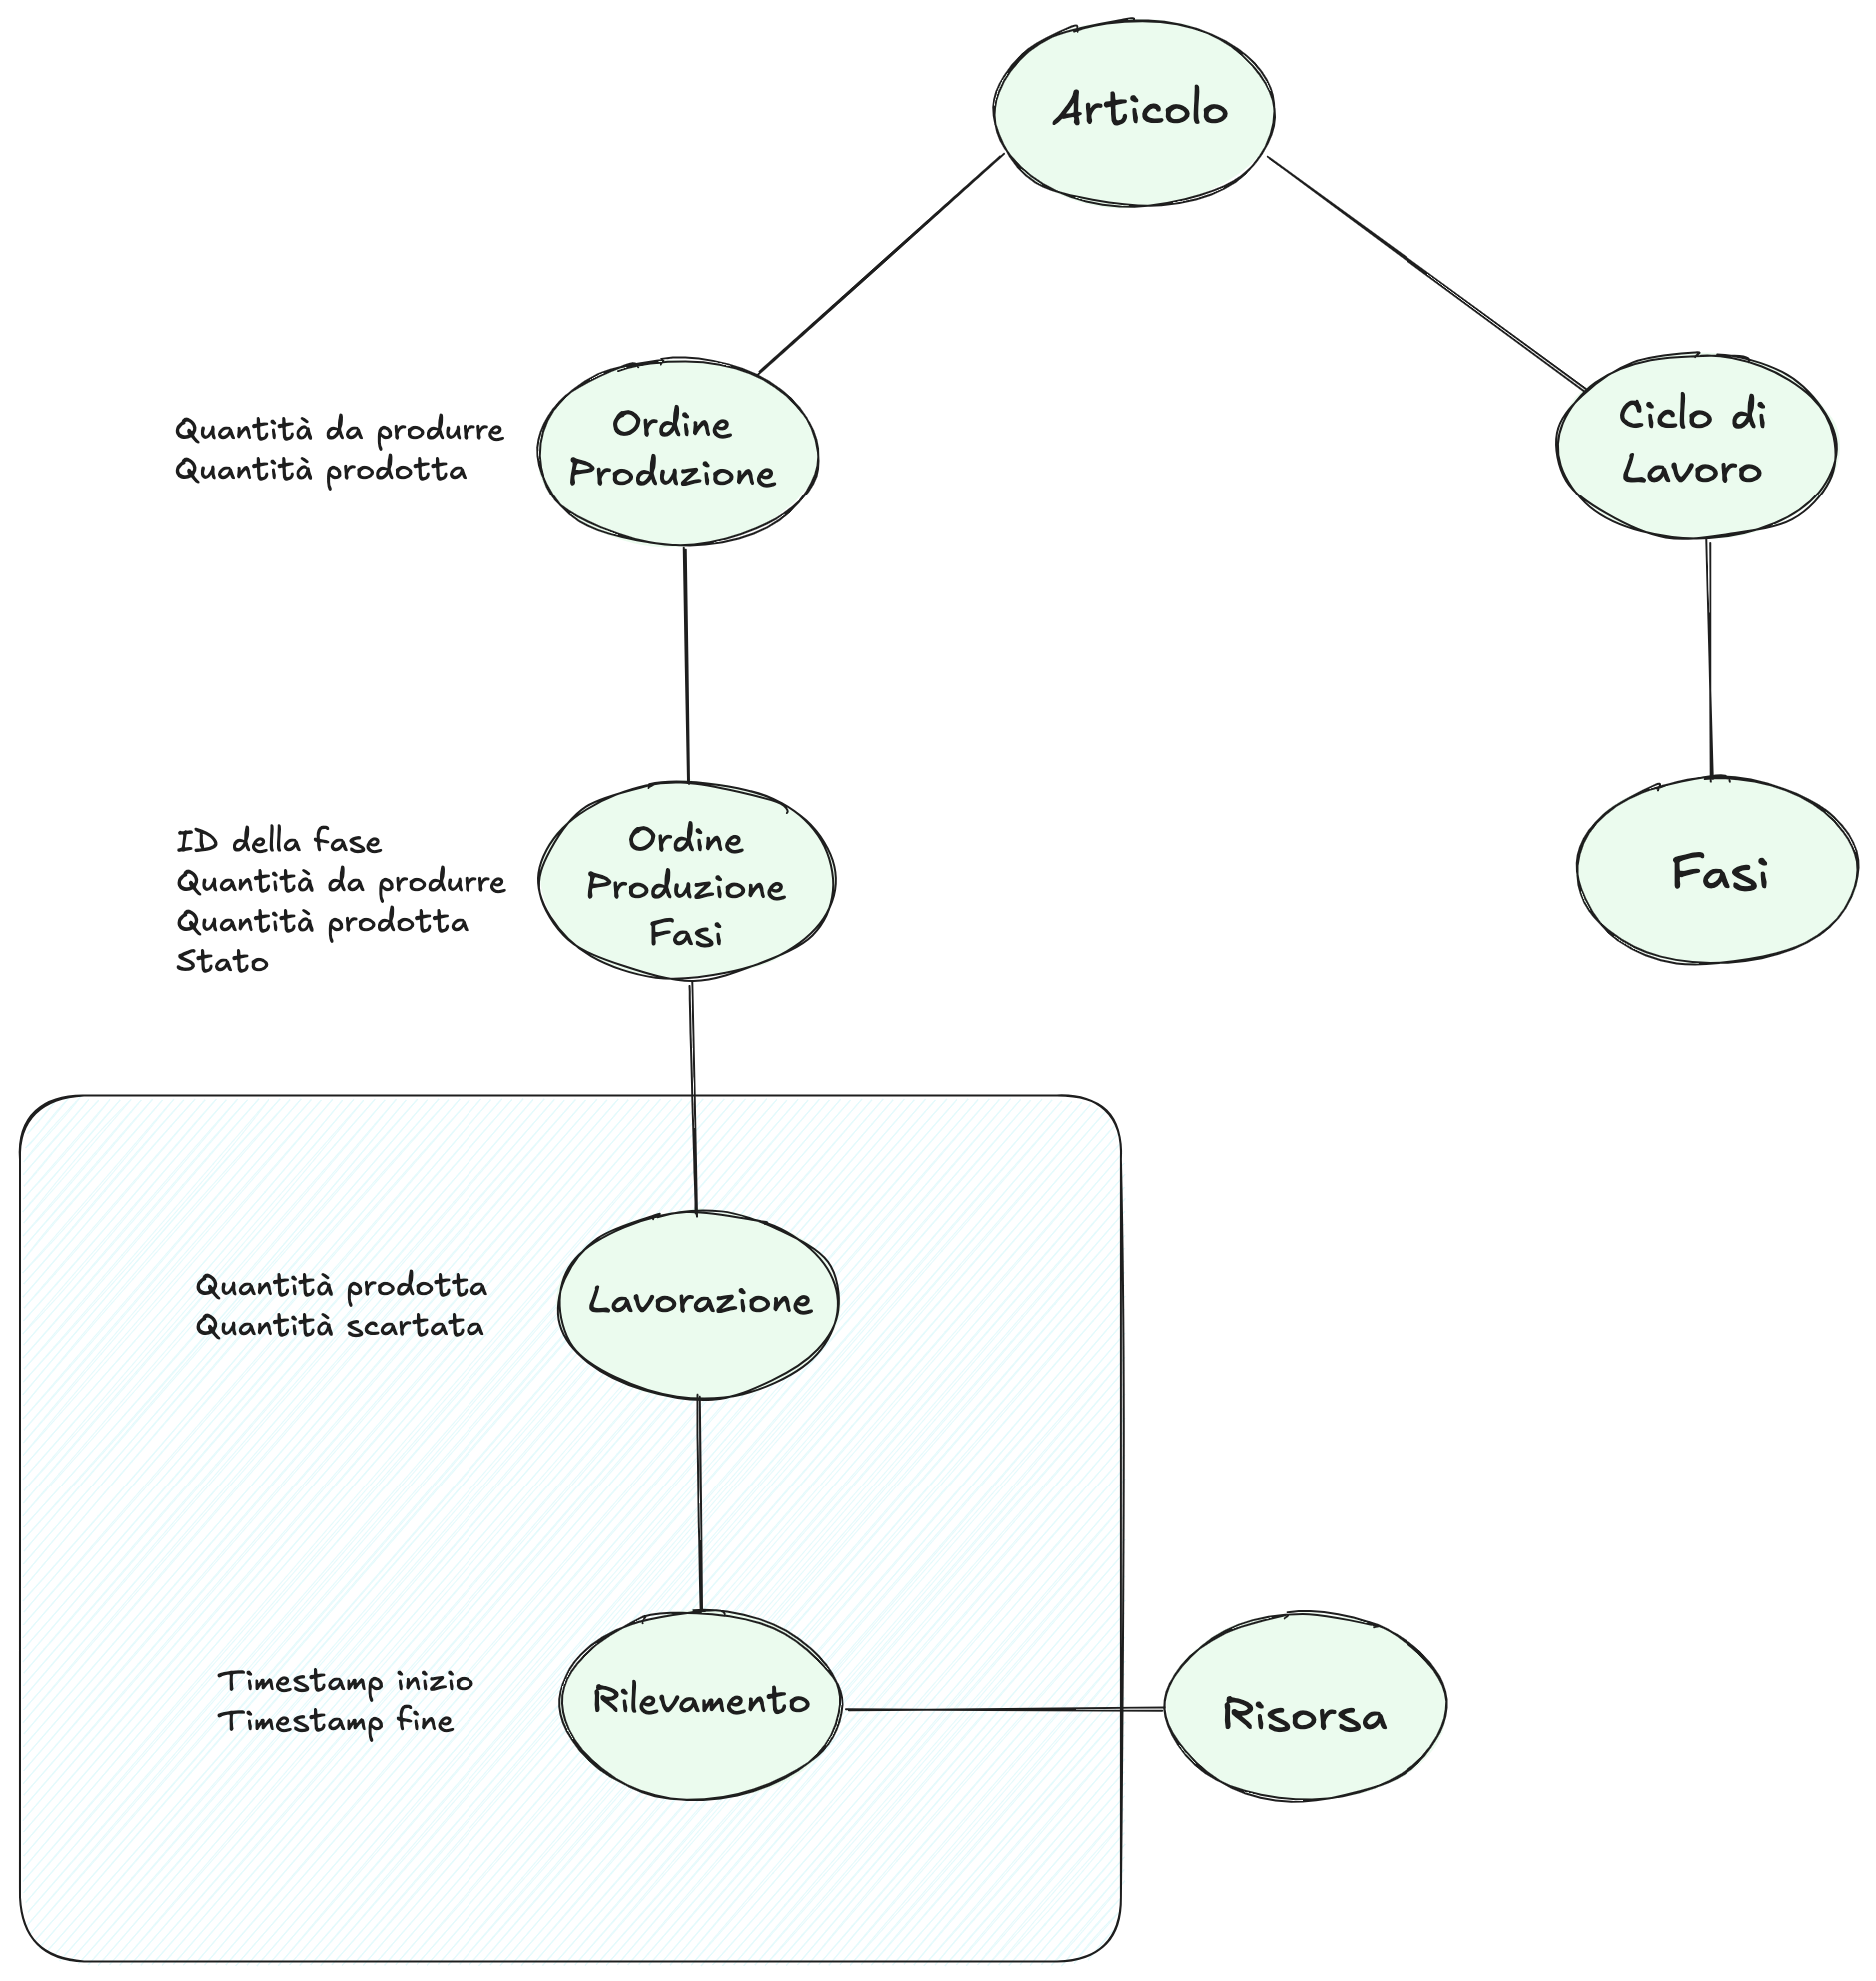
\includegraphics[width=0.6\linewidth]{BCS-Tessi//images/Dominio.png}
            \caption[Modello di dominio preso in esame]{Schema visuale del modello di dominio preso in esame durante l'attività di analisi dei requisiti}
            \label{fig:Dominio}
        \end{figure}

        \vspace{0.2 em}
        \noindent L'immagine descrive una situazione reale semplificata con cui l'azienda si interfaccia: la gestione della produzione di un certo \texttt{Articolo} finito, la cui produzione prevede un certo \texttt{CicloDiLavoro} composto da diverse \texttt{Fasi} che sono predefinite. Consideriamo ogni componente corrispondere a un \textit{bounded context}.
        Nello specifico: 
        \begin{itemize}
            \item La produzione di un \texttt{Articolo} richiede un \texttt{OrdineProduzione}, che rappresenta la quantità da produrre e la quantità prodotta.
            \item \texttt{OrdineProduzioneFasi} tiene traccia dello stato di avanzamento della produzione considerando quante unità sono state prodotte in base alla \texttt{Fase} e anche in base ai materiali disponibili. Può infatti succedere che la quantità richiesta non venga raggiunta per mancanza di materiali sufficienti: il conteggio si ferma automaticamente quando il numero di unità è stato raggiunto o manualmente quando le risorse sono state esaurite. Tiene conto della quantità da produrre, della quantità prodotta e dello stato (aperto, in corso, chiuso).
            \item Il riquadro nell'immagine comprende i \textit{bounded context} presi in analisi. Il \texttt{Rilevamento} prevede che ogni lavoratore segnali (attraverso un \textit{badge}) al sistema il momento di inizio del lavoro e il momento della fine dello stesso, con il numero di pezzi prodotti in base alla fase di lavoro corrispondente. Il completamento di una fase di \texttt{Rilevamento} fa avanzare anche \texttt{Lavorazione} che tiene conto della quantità prodotta e della quantità scartata.
            \item Una \texttt{Risorsa} è rappresentata dall'operaio, la macchina che utilizza per la fase determinata, la \texttt{Fase}, il numero di unità prodotte, l'ora di inizio del lavoro e l'ora di fine.
        \end{itemize}

        \vspace{0.2 em}
        \noindent Il problema principale è far comunicare in tempo reale \texttt{Rilevamento} e \texttt{OrdineProduzioneFasi}, senza che quest'ultimo debba essere portato all'interno del microservizio che individuiamo come \texttt{MS\_Rilevamento}.

        \vspace{0.2 em}
        \noindent La soluzione ideale infatti sarebbe quella di includere \texttt{OrdineProduzione} e \texttt{OrdineProduzioneFasi} nell'unico microservizio \texttt{MS\_Rilevamento}. Questo perché secondo i principi del \textit{Domain-Driven Design} la divisione in \textit{bounded contexts} dovrebbe attuare una scomposizione in microservizi che siano poco accoppiati tra di loro. In questo caso invece c'è un alto grado di accoppiamento tra i \textit{bounded context} appena citati e  \texttt{Lavorazione}, quindi scomporli in servizi differenti non è in linea con i principi DDD\footnote{E. Evans, Domain-Driven Design: Tackling Complexity in the Heart of Software, Addison-Wesley, 2003}.

        \vspace{0.2 em}
        \noindent Questa soluzione non è applicabile al momento perché il monolite è strettamente collegato in vari punti con \texttt{OrdineProduzione} e con \texttt{OrdineProduzioneFasi}. La priorità è dunque estrarre \texttt{Rilevamento} e \texttt{Lavorazione} in un unico servizio, e in un secondo momento completare la divisione ideale.

        \vspace{0.2 em}
        \noindent Inoltre, un altro problema è rappresentato dalla necessità di \texttt{MS\_Rilevamento} di leggere dei dati da due fonti. Per monitorare lo stato di una \texttt{Lavorazione} in relazione a \texttt{OrdineProduzione}, è necessario confrontare i dati provenienti sia dal microservizio, sia dal monolite. Questo perché altrimenti non è possibile accedere ai dati essenziali dell'ordine della fase da lavorare, senza portare \texttt{OrdineProduzione} all'interno di \texttt{MS\_Rilevamento}. Come farlo sarà oggetto della sezione successiva. 

        \subsection{Progettazione}
        Durante il mio \textit{stage}, l’analisi dei requisiti e la fase di progettazione si sono sviluppate in modo parallelo. Con l’aumentare della mia conoscenza del dominio applicativo e l’individuazione dei requisiti, la progettazione, guidata dal \textit{Product Owner}, è avvenuta in modo naturale, senza una netta separazione tra le due attività.  

        \vspace{0.2 em}
        \noindent Poiché la progettazione consiste nel definire come realizzare concretamente quanto emerso dall’analisi dei requisiti, questo capitolo si concentrerà sulla descrizione dei \textit{pattern} identificati e delle soluzioni architetturali adottate per soddisfare i requisiti individuati.

        \vspace{0.2 em}
        \noindent La soluzione individuata è rappresentata nella Figura \ref{fig:progettazione} e rappresenta il modo in cui \texttt{MS\_} \texttt{Rilevamento} potrà comunicare con SAI attraverso un \texttt{MS\_Middleware}. Questo rappresenta molto bene il piano di migrazione visibile nella Figura \ref{fig:migrazione}.
        
        \begin{figure}
            \centering
            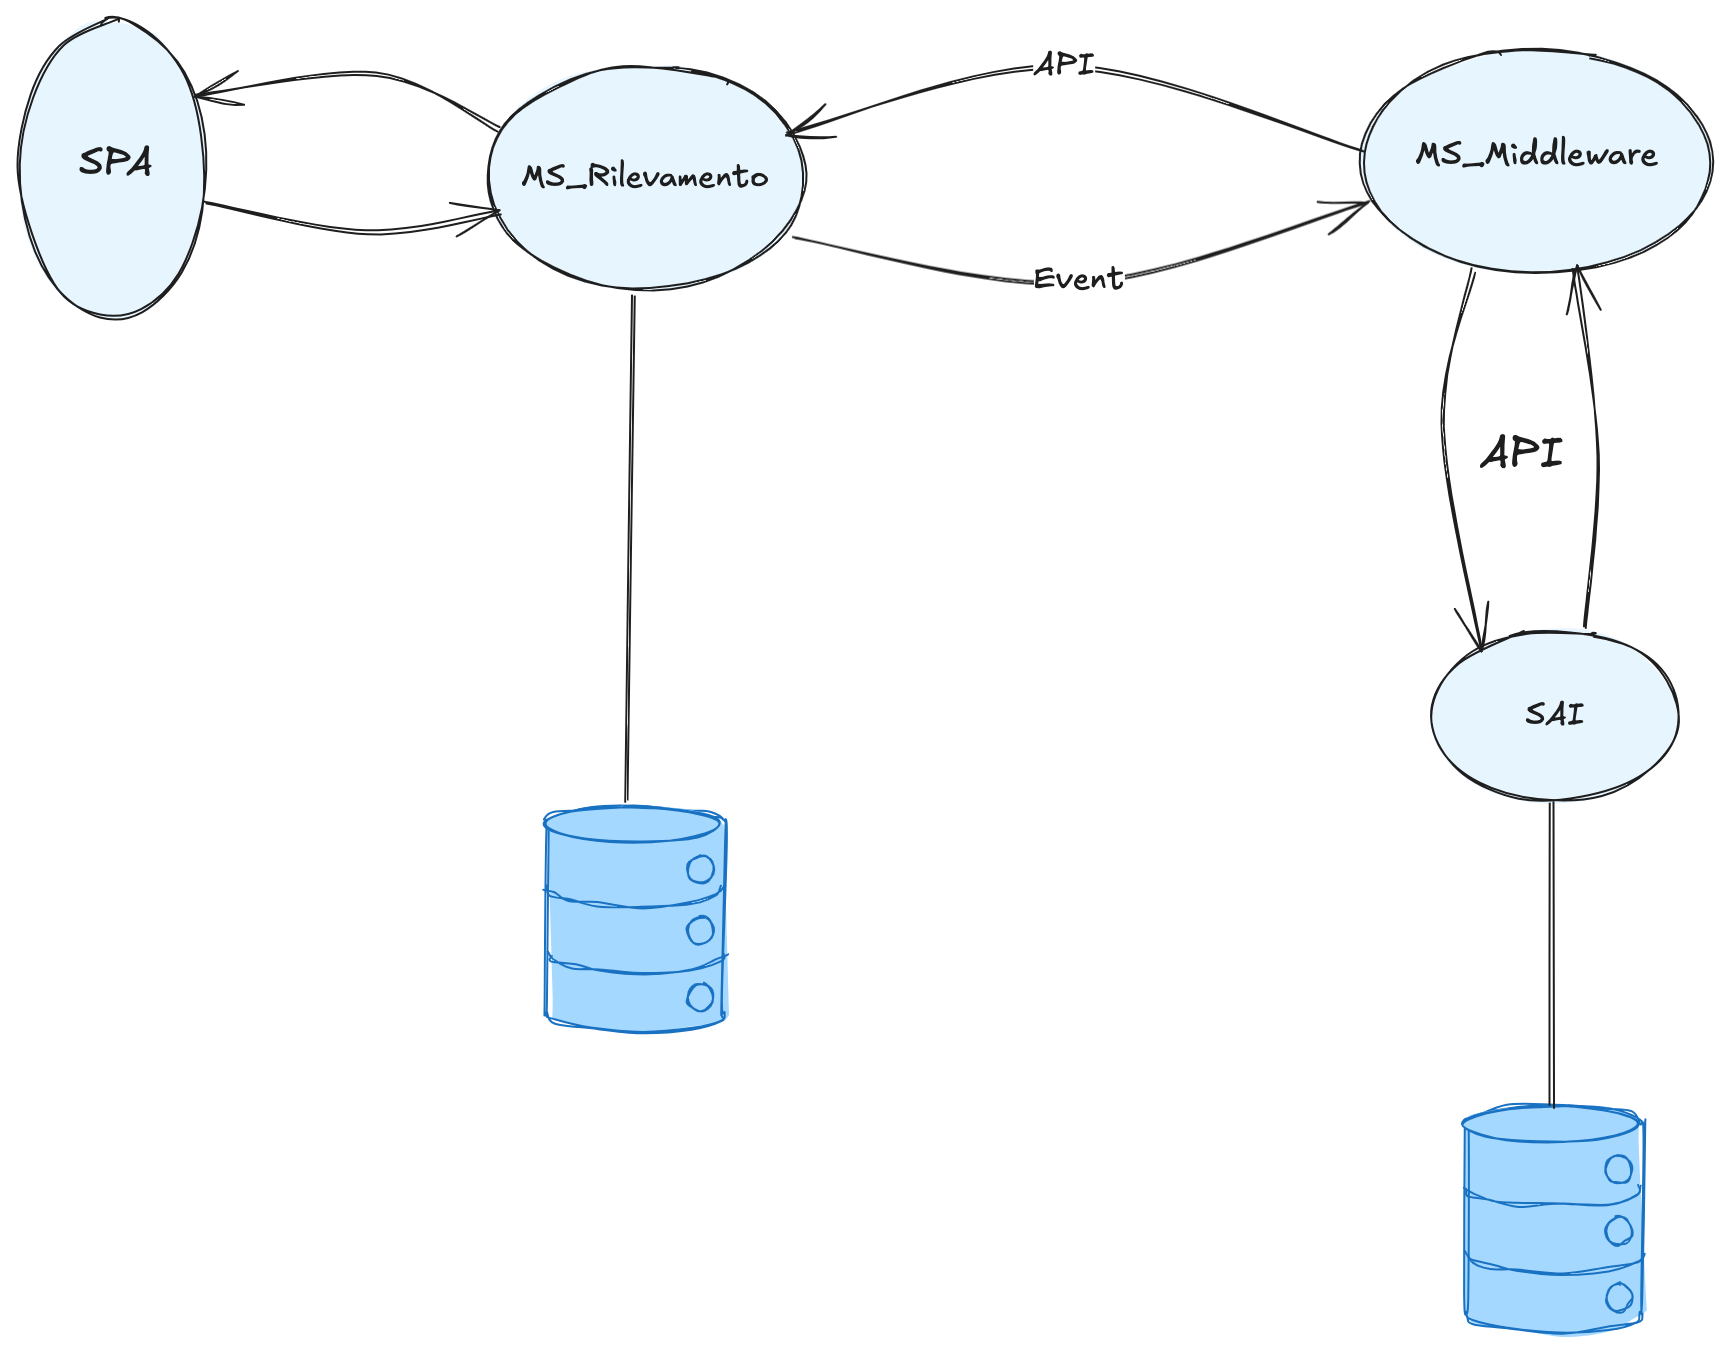
\includegraphics[width=0.6\linewidth]{BCS-Tessi//images/Progettazione.png}
            \caption[Progettazione per l'estrazione del microservizio]{Attività di progettazione per quanto concerne l'estrazione di \texttt{MS\_Rilevamento}}
            \label{fig:progettazione}
        \end{figure}

        \vspace{0.2 em}
        \noindent Date le dimensioni molto grandi del monolite in esame, l'azienda ha scelto di optare per una migrazione graduale. La soluzione più ragionevole è risultata dunque quella di applicare il \textit{pattern} \textit{Anti-Corruption Layer} (ACL) prevedendo la lunga convivenza del monolite e del nuovo sistema a microservizi. 

        \vspace{0.2 em}
        \noindent Un altro \textit{pattern} che ho proposto è il \textit{Change Data Capture}, una tecnica utilizzata per identificare e tracciare le modifiche apportate ai dati in un database. Nel nostro caso è utile nei contesti di sincronizzazione tra sistemi eterogenei, ossia di \texttt{MS\_Rilevamento} e di SAI, il monolite. 

        \vspace{0.2em}
        \noindent Per l'implementazione di questo microservizio, insieme al \textit{Product Owner} siamo giunti alla scelta del modello di \textbf{architettura esagonale}, noto anche come \textit{pattern} di porte e adattatori che mira a creare architetture liberamente accoppiate in cui i componenti delle applicazioni possano essere testati in modo indipendente, senza dipendenze da archivi di dati o interfacce utente. Viene utilizzato per isolare la logica aziendale (logica di dominio) dal codice dell'infrastruttura correlato. Le \textbf{porte} sono punti di ingresso indipendenti dalla tecnologia in un componente dell'applicazione. Gli \textbf{adattatori} invece, implementano le interfacce definite dalle porte, consentono una comunicazione fluida tra il nucleo applicativo e i sistemi esterni, facilitando future estensioni o sostituzioni di componenti senza impattare sulla logica di business centrale.

        \vspace{0.2 em}
        \noindent Come anticipato nella precedente sezione, un problema da risolvere era quello di effettuare due letture sul \textit{bounded context} \texttt{Lavorazione}. La soluzione trovata per fare ciò è effettuare una lettura su \texttt{MS\_Rilevamento} tramite un \textit{adapter} PostgreSQL sul \textit{database} locale, e una su SAI tramite una connessione PostgreSQL al \textit{database} del monolite stesso. Studiando i \textit{pattern} di scomposizione dei \textit{database}, per questa specifica situazione ho individuato il pattern \textbf{\textit{Database Wrapping Service}}\footnote{S. Newman, Monolith to Microservices: Evolutionary Patterns to Transform Your Monolith, O'Reilly Media, 2019}. Nello specifico si implementa un servizio intermedio (\textit{wrapping service}) che si occupa di esporre le informazioni di SAI tramite delle \textit{Web} API senza esporre direttamente il \textit{database} sottostante. 

        \vspace{0.2 em}
        \noindent In questo modo, il \textit{team} che gestisce il monolite è responsabile dell’aggiornamento delle API in caso di modifiche alla struttura del \textit{database}, e il \textit{team} di \texttt{MS\_Rilevamento} non deve preoccuparsi dei cambiamenti interni a SAI. Questo approccio riduce l'accoppiamento tra i sistemi, rendendo più facile l'evoluzione della struttura dei dati.

        \vspace{0.2 em}
        \noindent Infine, insieme al \textit{Product Owner}, abbiamo pensato a come sincronizzare questi dati. Dallo studio della letteratura sui \textit{pattern} è emerso come migliore per il nostro problema il \textit{\textbf{Change Data Capture}} \textbf{(CDC)} implementato con un \textbf{\textit{Batch Delta Copier}}\ap{3}. 
        
        
        \vspace{0.2 em} 
        \noindent Il \textit{Change Data Capture} è un \textit{pattern} che monitora e cattura le modifiche ai dati in un sistema di origine (nel nostro caso SAI) per sincronizzarle con sistemi di destinazione, garantendo così la coerenza delle informazioni attraverso piattaforme diverse. Il \textit{Batch Delta Copier} è un'implementazione specifica di CDC che funziona identificando periodicamente i dati nuovi o modificati dalla sorgente (il "delta") e copiandoli in blocco verso la destinazione durante finestre temporali programmate.


        
        \subsection{Implementazione}
        La fase di progettazione è stata senza dubbio la più complessa, soprattutto a causa della mancanza di soluzioni definitive e della relativa novità del concetto di migrazione verso i microservizi. Nonostante le difficoltà iniziali, una volta definita la strategia da adottare, l’implementazione è proseguita in modo naturale, seguendo il percorso tracciato.  

        \vspace{0.2 em}
        \noindent La fase di codifica è stata improntata su un approccio \textit{learn by doing}: pur avendo una base di riferimento, ho dovuto affinare le mie competenze sul campo, confrontandomi regolarmente con il \textit{tutor} aziendale e il \textit{Product Owner} per ricevere \textit{feedback} e indicazioni utili.
        
        \noindent Nello specifico, ho potuto implementare una struttura di progetto molto precisa, rappresentata nella Figura \ref{fig:code-structure}.

         
        \begin{figure}
            \centering
            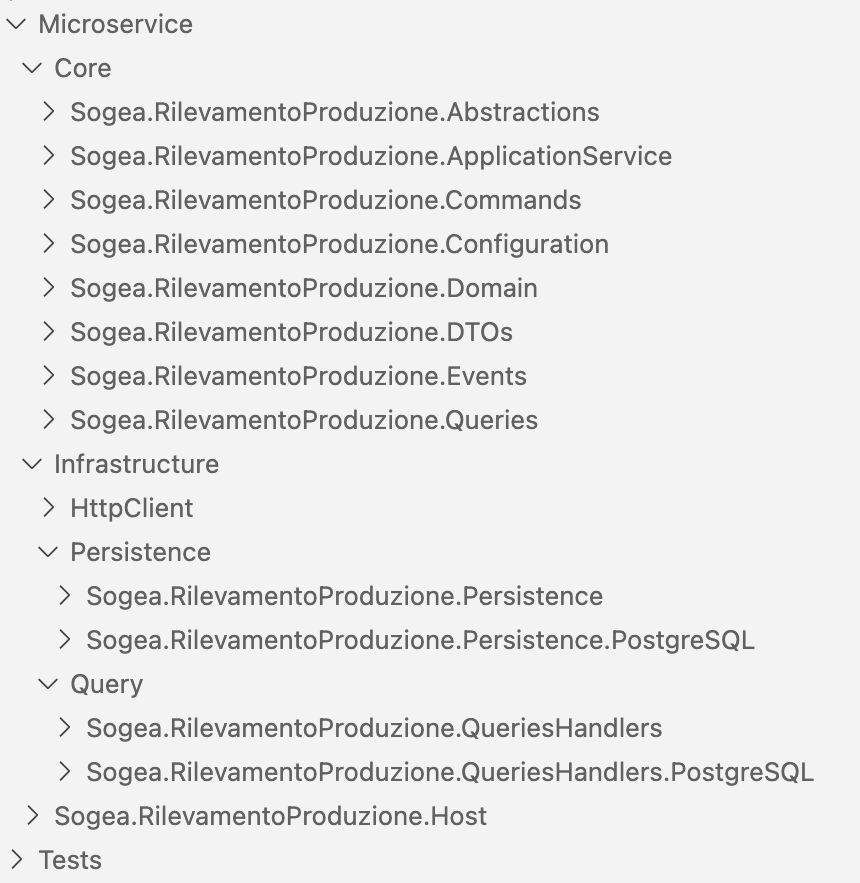
\includegraphics[width=0.5\linewidth]{BCS-Tessi//images/code_structure.png}
            \caption{Struttura del codice utilizzata per l'estrazione del microservizio.}
            \label{fig:code-structure}
        \end{figure}

        \vspace{0.2 em}
        \noindent Analizzando più approfonditamente la struttura del microservizio \texttt{Sogea.Rilevamento}\texttt{Produzione}, posso espandere i seguenti concetti architetturali:
        \begin{itemize}
            \item \textbf{\textit{Domain-Driven Design}} \textbf{(DDD)}: il microservizio implementa i principi DDD attraverso la separazione in \textit{$namespace_G$} come \texttt{Domain}, \texttt{Abstractions}. Mentre \texttt{Domain} contiene le entità di dominio e gli aggregati, le \texttt{Abstraction} forniscono interfacce che definiscono comportamenti senza implementazioni concrete;
            \item \textbf{\textit{Command Query Responsibility $\textbf{Segregation}_G$} (CQRS)}: è un modello architetturale che separa le operazioni di lettura (\textit{query}) da quelle di scrittura (comandi) utilizzando interfacce distinte per ottimizzare le prestazioni e la scalabilità.I \texttt{Commands} gestiscono le operazioni di scrittura e la modifica dello stato, mentre le \texttt{Queries} gestiscono le operazioni di lettura. I \texttt{QueryHandlers} elaborano le \textit{query} e interagiscono con PostgreSQL;
            \item \textbf{\textit{Event Sourcing}}: il \textit{namespace} \texttt{Events} indica l'implementazione di Event Sourcing,  modello architetturale che memorizza lo stato di un sistema come una sequenza di eventi immutabili, permettendo di ricostruire lo stato corrente riproducendo tali eventi.
            \item \textbf{\textit{Data Transfer Objects} (DTOs)}: il \textit{namespace} \texttt{DTOs} (\texttt{Sogea.RilevamentoProduzione.}\texttt{ DTOs}) contiene oggetti utilizzati per trasferire dati tra i diversi livelli dell'applicazione. I DTOs sono oggetti immutabili che incapsulano dati per il trasferimento tra componenti;
            \item \textbf{\textit{Handlers}}: gli \texttt{Handlers} rappresentano il punto di contatto tra l'infrastruttura e il dominio, traducendo le richieste in operazioni sul dominio e sono rappresentativi dell'applicazione dell'architettura esagonale.
        \end{itemize}

        \vspace{0.2 em}
        \noindent I microservizi, per loro natura intrinseca, comportano significative attività di integrazione per garantire una comunicazione efficace tra i diversi componenti. Un esempio concreto di questa necessità è rappresentato dalla soluzione implementata per il problema, presentato nelle sezioni immediatamente precedenti, della duplice lettura, che si verificava sia sul sistema monolitico sia sul microservizio \texttt{MS\_Rilevamento}. Per risolvere questa criticità, è stata sviluppata un'\textbf{API} dedicata che funge da intermediario nella comunicazione, ottimizzando così il flusso di dati tra le diverse parti dell'architettura.

        \begin{verbatim}
        public async Task<OrdineProduzione> FindByFaseAsync(int ordineProduzioneFaseId)
        {
          string url = this.Configuration.Server.Replace("{productionOrderId}", 
          ordineProduzioneFaseId.ToString());
          RestClient client = new RestClient(url);
          RestRequest request = new RestRequest(Method.GET);
          request.AddHeader("DITTA", this.Configuration.Ditta);
          IRestResponse response = await client.ExecuteAsync(request);
          if (response.IsSuccessful && response.Content != null)
          {
            RootDto rootDto = JsonConvert.DeserializeObject<RootDto>(response.Content);
            // ... elaborazione della risposta ...
          }
          return null;
        }
        \end{verbatim}

        \vspace{0.2 em}
        \noindent Il componente fondamentale che implementa l'operazione di lettura all'interno dell'API è il metodo \texttt{FindByFaseAsync} della classe \texttt{OrdineProduzioneRepository}. Questo metodo esemplifica l'implementazione di un'operazione di recupero dati (Read) secondo il paradigma $REST_G$, approfondito nella Sezione 1.7.

        \vspace{0.2 em}
        \noindent L'operazione di lettura si articola attraverso i seguenti passaggi:
        \begin{itemize}
            \item \textbf{costruzione dell'\textit{$\textbf{endpoint}_G$}}: l'$URL_G$ di destinazione viene dinamicamente generato sostituendo il parametro \texttt{productionOrderId} con l'identificativo della fase di produzione richiesta;
            \item \textbf{configurazione della richiesta $HTTP_G$}: viene istanziato un \textit{client} REST e configurata una richiesta di tipo GET, che per definizione nel protocollo HTTP rappresenta un'operazione di lettura non modificante;
            \item \textbf{contestualizzazione della richiesta}: \texttt{DITTA} viene aggiunto per specificare il contesto aziendale della richiesta, consentendo al servizio di rispondere con i dati pertinenti.
            \item \textbf{esecuzione asincrona}: a richiesta viene eseguita in modalità asincrona (\texttt{await client.} 
            \texttt{ExecuteAsync}), ottimizzando l'utilizzo delle risorse del sistema durante l'attesa della risposta;
            \item \textbf{elaborazione dei dati}: in caso di risposta positiva, i dati $JSON_G$ ricevuti vengono deserializzati e trasformati in oggetti del dominio applicativo.
        \end{itemize}

        \vspace{0.2 em}
        \noindent Per affrontare invece la problematica della sincronizzazione dei dati, ho potuto esplorare e implementare un'architettura specializzata basata sulla tecnologia \textbf{Debezium}, una piattaforma di \textbf{\textit{Change Data Capture}} (\textbf{CDC}), approfondita nella Sezione 1.7. 

        \vspace{0.2 em}
        \noindent L'architettura di sincronizzazione adottata ha integrato Debezium con \textbf{RabbitMQ}, quest'ultimo utilizzato come \textit{message broker }per la gestione efficiente del flusso di informazioni. Questa combinazione tecnologica ha consentito la realizzazione di un sistema di code (inteso come liste) di messaggi altamente reattivo, in grado di catturare e propagare le modifiche ai dati nel momento stesso in cui queste venivano apportate nel sistema di origine.

        \vspace{0.2 em}
        \noindent Il principio operativo di questa soluzione si basa sul meccanismo di CDC, attraverso il quale Debezium monitora continuamente il \textit{log} delle transazioni del \textit{database}, identifica le operazioni di inserimento, aggiornamento o eliminazione dei dati e trasforma queste informazioni in eventi che vengono successivamente instradati attraverso RabbitMQ verso i sistemi destinatari, come si può osservare in Figura \ref{fig:queue}.

        \begin{figure}[H]
            \centering
            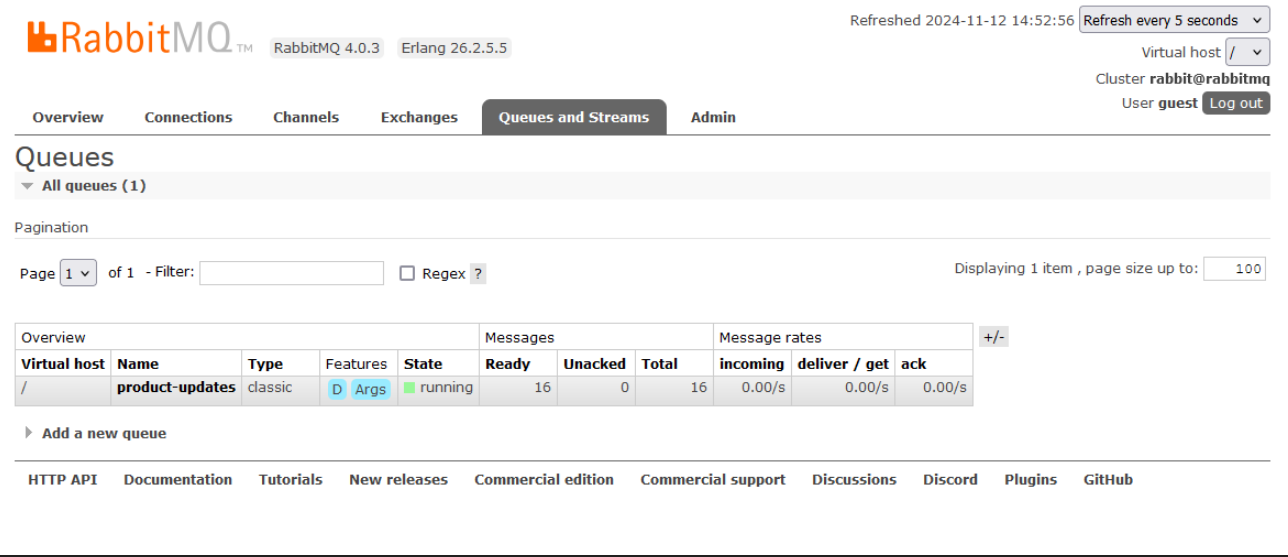
\includegraphics[width=1\linewidth]{BCS-Tessi//images/queue.PNG}
            \caption{Coda implementata con Debezium e gestita da RabbitMQ.}
            \label{fig:queue}
        \end{figure}

        
        \subsection{Verifica e validazione}
        Durante il processo di sviluppo, ho adottato un approccio sistematico all'implementazione dei \textit{test} unitari, integrandoli organicamente nel ciclo di sviluppo iterativo. L'esecuzione dei \textit{test} unitari avveniva contestualmente all'implementazione di nuove funzionalità, seguendo la metodologia di sviluppo incrementale. Questo mi ha permesso di attuare una copertura totale di \textit{test} del codice.

        \vspace{0.2 em}
        \noindent Le sessioni di \textit{Sprint Review} costituivano un momento di verifica, durante il quale le funzionalità sviluppate erano sottoposte a un processo di validazione che coinvolgeva anche il \textit{Product Owner}, garantendo così la verifica della conformità rispetto ai requisiti iniziali.

        \vspace{0.2 em}
        \noindent Inoltre, ho eseguito ulteriori verifiche di integrazione per assicurare la corretta esposizione delle funzionalità sviluppate nell'ambiente \textit{server}. A tal fine, ho utilizzato Swagger come strumento primario di verifica e documentazione delle API. Questo \textit{framework}, approfondito nella Sezione 1.7, mi ha permesso di visualizzare in tempo reale l'effettivo funzionamento delle nuove implementazioni, offrendo un'interfaccia intuitiva per l'interazione con i servizi esposti, il cui funzionamento è osservabile nella Figura \ref{fig:swagger}.
        
        \begin{figure}[H]
            \centering
            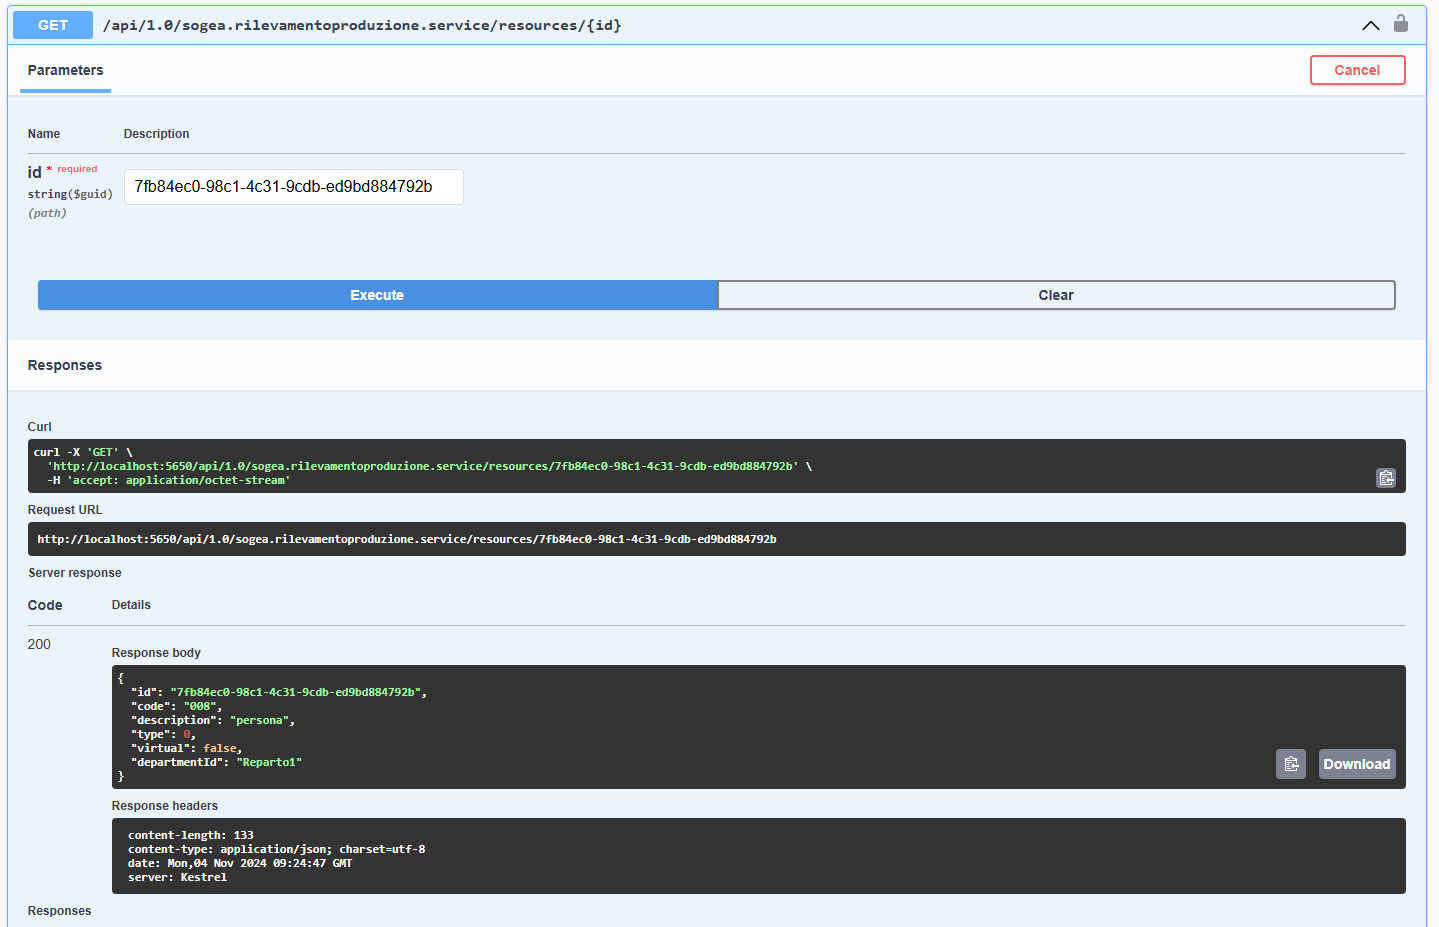
\includegraphics[width=1\linewidth]{BCS-Tessi//images/swagger.PNG}
            \caption{Swagger}
            \label{fig:swagger}
        \end{figure}

        \vspace{0.2 em}
        \noindent Come anticipato nella Sezione 1.6.4, il processo di Validazione fornisce evidenza oggettiva sulle capacità del \textit{software} di soddisfare le aspettative e i bisogni del committente. 

        \vspace{0.2 em}
        \noindent Data la natura accademica del mio \textit{stage}, non si sono svolte validazioni più formali che avrebbero incluso il coinvolgimento di \textit{stakeholder} esterni.

        \vspace{0.2 em}
        \noindent Nel mio caso infatti, il processo di validazione è stato caratterizzato da un approccio collettivo, coinvolgendo diverse figure all'interno dell'organizzazione. La responsabilità primaria di tale validazione è stata assunta dal \textit{Product Owner} e dal \textit{Team Leader}, che ha supervisionato gli aspetti tecnici dell'implementazione. Durante una \textit{Sprint Review}, ho presentato le funzionalità implementate e il loro funzionamento a tutto il \textit{team} di sviluppo che interagisce con questo particolare microservizio.


    \section{Risultati raggiunti}
        \subsection{Il microservizio}
        Descriverò le funzionalità del servizio estratto e l'efficacia dell'aggiornamento dei dati con il monolite.
        Scriverò una visione qualitativa degli obiettivi raggiunti, il loro allineamento al modello di dominio individuato.

        L'operazione di estrazione del microservizio dal sistema monolitico preesistente ha raggiunto l'obiettivo prefissato, conseguendo il risultato fondamentale di preservare integralmente le funzionalità originarie pur trasferendole in un'architettura indipendente. L'esito positivo di questa migrazione architetturale è evidenziato dalla piena operatività del componente estratto, ora funzionante come entità autonoma al di fuori del contesto monolitico in cui era originariamente integrato.
È doveroso precisare che il processo di estrazione ha richiesto l'implementazione di soluzioni tecniche che, sotto il profilo dell'eleganza architetturale, potrebbero essere considerate sub-ottimali. Tuttavia, tali compromessi sono stati consapevolmente accettati in considerazione dell'obiettivo primario del progetto, che consisteva nell'estrazione funzionale del microservizio piuttosto che nella realizzazione di un'architettura ideale dal punto di vista teorico.
Al termine del periodo di stage, il microservizio estratto ha raggiunto un livello di autonomia operativa significativo, pur mantenendo specifici canali di comunicazione con il sistema monolitico originario per garantire la continuità dei processi aziendali. Questa configurazione ha consentito al microservizio di assumere la responsabilità esclusiva della gestione dei rilevamenti e delle lavorazioni associate alle fasi produttive, interfacciandosi con il sistema di gestione degli ordini di produzione e delle relative fasi.
Come illustrato nella documentazione grafica di riferimento, l'architettura risultante dimostra la capacità del microservizio di operare come componente indipendente all'interno dell'ecosistema applicativo complessivo, rappresentando un significativo passo avanti nel processo di decomposizione del monolite verso un'architettura orientata ai microservizi.

        \begin{figure}[H]
            \centering
            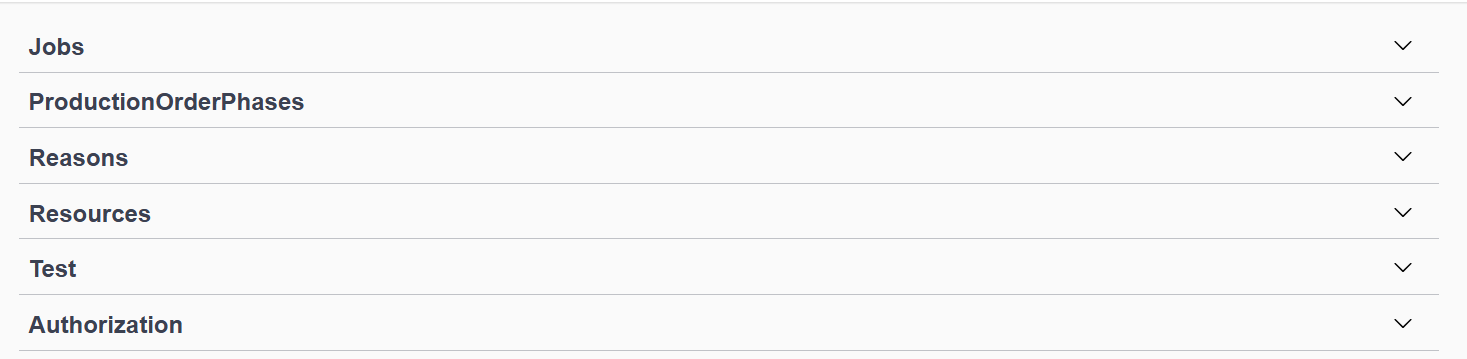
\includegraphics[width=1\linewidth]{BCS-Tessi//images/FinalSwagger.PNG}
            \caption{Final Swagger}
            \label{fig:final-Swagger}
        \end{figure}
        
        L'estrazione del microservizio ha prodotto un significativo miglioramento nell'efficienza operativa dell'organizzazione, risolvendo problematiche strutturali che affliggevano il sistema precedente. La transizione architetturale ha permesso di superare le limitazioni imposte dall'approccio precedentemente adottato, basato sul pattern "batch delta copier", che rappresentava un significativo collo di bottiglia nei flussi informativi aziendali.
Nella configurazione precedente, l'aggiornamento dei dati avveniva attraverso procedure batch eseguite con cadenza giornaliera, imponendo un ritardo sistematico di 12 ore nella disponibilità delle informazioni aggiornate. Questa latenza costituiva un ostacolo significativo per gli operai, che si trovavano a lavorare con dati non allineati alla situazione corrente, compromettendo potenzialmente l'efficacia dei processi decisionali e operativi.
L'implementazione della tecnologia Debezium ha rivoluzionato questo paradigma, introducendo un meccanismo di aggiornamento in tempo reale che elimina la latenza informativa. Questo cambiamento ha permesso ai lavoratori di accedere immediatamente ai dati aggiornati, senza dover attendere l'esecuzione delle procedure batch notturne, con un conseguente incremento della reattività operativa e della qualità delle decisioni basate su informazioni tempestive.
È importante sottolineare che questa transizione verso un modello event-driven comporta un inevitabile compromesso in termini di consumo di risorse computazionali. La maggiore reattività del sistema si traduce in un più intenso utilizzo dell'infrastruttura IT, richiedendo un bilanciamento attento tra benefici operativi e costi infrastrutturali. In considerazione di questo trade-off, l'implementazione della sincronizzazione in tempo reale è stata strategicamente limitata ai soli dati per i quali la tempestività dell'aggiornamento rappresenta un requisito critico per i processi aziendali, ottimizzando così l'allocazione delle risorse disponibili.

        
        \subsection{Risultati quantitativi}
        Descriverò i risultati quantitativi raggiunti: sia riguardo alla documentazione effettivamente scritta, al codice sviluppato, eventuali \textit{report} e diagrammi, sia riguardo al miglioramento della \textit{performance} del sistema in generale, il \textit{tradeoff} tra miglioramenti e rallentamenti, in base agli obiettivi del progetto (e quindi del dominio).

        Durante il periodo di stage, ho conseguito con successo tre dei quattro obiettivi obbligatori inizialmente concordati, unitamente all'obiettivo facoltativo. L'obiettivo classificato come "desiderabile" non è stato affrontato, in seguito a una riconfigurazione strategica delle priorità progettuali. Tale riallineamento ha privilegiato lo sviluppo di una Proof of Concept (PoC), identificata come attività facoltativa (FA1), rispetto alla documentazione esaustiva dell'ecosistema dei servizi preesistenti e delle loro interdipendenze (OB3).
Questa riprioritizzazione delle attività si è rivelata funzionale al rispetto del vincolo temporale delle 304 ore allocate per l'esperienza formativa. L'efficiente gestione del tempo ha inoltre consentito l'estensione delle attività oltre il perimetro inizialmente definito, permettendo la realizzazione di un prototipo funzionale che rappresenta l'evoluzione naturale della Proof of Concept sviluppata.
I risultati tangibili prodotti durante il periodo di stage comprendono:

Un elaborato di analisi della letteratura scientifica concernente le metodologie di migrazione verso architetture a microservizi
Un documento tecnico sui pattern di migrazione, con particolare enfasi sugli approcci ritenuti più pertinenti per il contesto specifico di SogeaSoft
Un'analisi formale dei requisiti che sintetizza le esigenze funzionali e non funzionali identificate
Un corpus di 5826 linee di codice sorgente, sottoposte a processi di verifica e successivamente integrate nel branch di sviluppo del progetto



        
    \section{Sviluppi futuri}
    Racconterò di quanto il mio progetto di stage sia rilevante per SogeaSoft S.r.l. rispetto al loro obiettivo di migrazione completa del loro sistema verso un'architettura a microservizi.

    Il progetto di stage da me intrapreso riveste una particolare rilevanza per SogeaSoft in quanto si inserisce in un contesto di crescente esigenza di innovazione e miglioramento continuo del sistema software SAIonWeb. In seguito all’acquisizione da parte di Bluenext, come descritto nella Sezione 1.1, l’applicativo è destinato a gestire un numero sempre maggiore di clienti. Questa evoluzione comporta la necessità di aggiornamenti più frequenti e tempestivi, nonché l’adattamento del software alle specifiche esigenze aziendali e al relativo dominio di riferimento.  

Un aspetto cruciale risiede nella capacità di garantire ai clienti l’accesso ai dati in tempo reale, superando l’attuale limite che impone tempi di attesa di 24 ore per ottenere i dati del giorno precedente. Per raggiungere tale obiettivo, risulta imprescindibile scomporre l’architettura monolitica esistente e procedere verso una migrazione a un’architettura basata su microservizi.  
Immagino che la prima cosa che caratterizzerà anche i progetti di stage futuri sarà l'approfondimento della tecnologia Debezium, proprio a questo proposito. 
Ma non solo, anche l'esplorazione di nuovi pattern, dato che per ogni bounded context può corrispondere un microservizio, dunque il lavoro da fare è ancora molto. 

Tuttavia, il processo di migrazione si presenta come un percorso complesso e articolato, principalmente a causa della natura stessa del monolite SAI, il quale risulta stratificato e accoppiato a seguito di anni di sviluppo e aggiornamenti continui. La trasformazione dell’architettura monolitica in un insieme di microservizi richiederà dunque un notevole sforzo organizzativo e tecnico, nonché una pianificazione accurata e progressiva.  

In tale contesto, il progetto di stage ha costituito un primo passo significativo verso l’obiettivo più ampio della migrazione completa. Pur rappresentando solo una parte del progetto di lungo termine, il lavoro svolto ha permesso di delineare e testare approcci metodologici e tecnici che potranno essere riutilizzati e ampliati nelle fasi successive. La mia attività ha quindi contribuito a gettare le basi per un percorso di trasformazione che, nel medio-lungo periodo, porterà a una maggiore flessibilità e scalabilità del sistema SAIonWeb.
    
    
    